%%%%%%%%%%%%%%%%%%%%%%%%%%%%%%%%%%%%%%%%%%%%%%%%%%%%%%%%%%%%%%%%%%%%%%%
\chapter{Load Cell Based Smart Weighing System Using ESP32 and HX711}

%%%%%%%%%%%%%%%%%%%%%%%%%%%%%%%%%%%%%%%%%%%%%%%%%%%%%%%%%%%%%%%%%%%%%%%

\section{Introduction}

Accurate weight measurement plays an important role in industrial automation, laboratories, healthcare, and smart manufacturing. In this project, a compact digital weighing system was developed using a \textbf{1~kg load cell}, an \textbf{HX711 precision amplifier}, an \textbf{ESP32 Dev Module}, and a \textbf{SH1106 OLED display} to perform real-time weight measurement. The primary objective was to develop the weighing system and experimentally evaluate the sensitivity of a low-capacity load cell.

A strain-gauge load cell generates only a small differential voltage proportional to the applied load, which cannot be measured directly by the ESP32. Therefore, the \textbf{HX711 24-bit amplifier and Analog-to-Digital Converter (ADC)} was used to amplify and digitize the sensor output. The ESP32 then applies calibration and tare correction, calculates the measured weight, and continuously displays the result on the OLED display.

To evaluate the measurement capability of the developed system, a practical sensitivity experiment was performed by gradually removing approximately \textbf{1~mL} of water from a container at regular intervals. Since the density of water is approximately \textbf{1~g/mL}, each removal produced a weight reduction of nearly \textbf{1~g}. The measured values were recorded after the display stabilized and compared with the expected weight to assess the sensitivity, stability, and repeatability of the system.

The developed prototype integrates the load cell, HX711 amplifier, ESP32, and OLED display into a compact weighing platform supported by a custom mechanical frame. The project provided practical experience in sensor interfacing, embedded programming, calibration, hardware integration, and experimental evaluation while demonstrating the suitability of the system for laboratory measurements and future IoT-based monitoring applications.
%%%%%%%%%%%%%%%%%%%%%%%%%%%%%%%%%%%%%%%%%%%%%%%%%%%%%%%%%%%%%%%%%%%%%%%

\section{Objectives}

The objectives of this project are as follows.

\begin{itemize}
\item To assemble a smart weighing system using a load cell, HX711 module, ESP32, and OLED display.
\item To fabricate a mechanical frame for mounting the load cell and weighing platform.
\item To interface the load cell with the ESP32 using the HX711 amplifier.
\item To develop firmware for weight measurement and OLED display.
\item To calibrate the weighing system for accurate measurements.
\item To evaluate the performance of the developed system through experimental testing.
\end{itemize}
%%%%%%%%%%%%%%%%%%%%%%%%%%%%%%%%%%%%%%%%%%%%%%%%%%%%%%%%%%%%%%%%%%%%%%%

\section{System Overview}

The proposed smart weighing system integrates a load cell, HX711 amplifier module, ESP32 development board, SH1106 OLED display, and a custom mechanical support frame to perform real-time weight measurement. The system converts the mechanical force applied to the weighing platform into an electrical signal, which is amplified, digitized, processed, and displayed as weight.

Figure~\ref{fig:blockdiagram} illustrates the overall architecture of the developed system. When a load is placed on the weighing platform, the load cell produces a small differential voltage proportional to the applied force. The HX711 module amplifies this signal and converts it into digital data before transmitting it to the ESP32 through a serial interface. The ESP32 processes the received data using a calibration factor to determine the corresponding weight and displays the measured value on the SH1106 OLED display in real time.

A custom mechanical frame was fabricated to securely mount the load cell and weighing platform, ensuring stable operation and proper force transfer during measurements.

% \begin{figure}[H]
% \centering
% 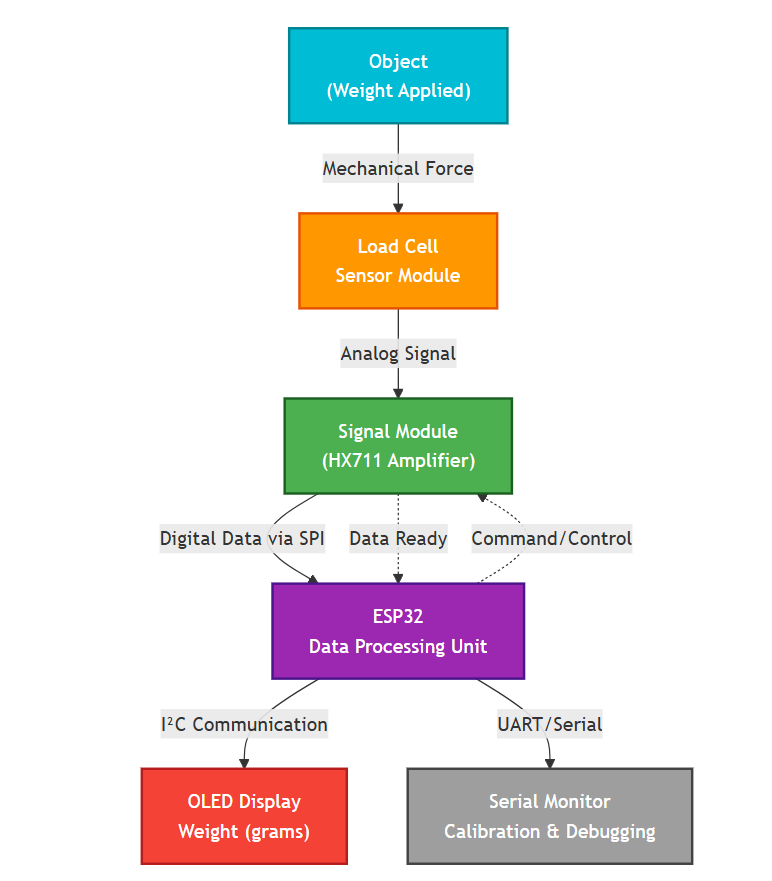
\includegraphics[width=0.65\textwidth]{projects_records/Load_cell/Images/system_block_diagram.png}
% \caption{Overall Architecture of the Load Cell-Based Smart Weighing System}
% \label{fig:blockdiagram}
% \end{figure}

\begin{figure}[H]
\centering
\resizebox{1\textwidth}{!}{%
\begin{circuitikz}
\tikzstyle{every node}=[font=\fontsize{22.8pt}{29.6pt}\selectfont]
\node [font=\fontsize{22.8pt}{29.6pt}\selectfont, inner xsep=0.080cm, inner ysep=0.085cm, rounded corners=0.020cm] at (11.5,11.875) {Load Cell → HX711 → ESP32 → OLED};
\draw  (3.75,13.125) rectangle (19.125,10.625);
\end{circuitikz}
}%
\caption{Flow diagram of the proposed load cell-based smart weighing system.}
\label{fig:blockdiagram}
\end{figure}




The signal flow begins with the applied load and continues through the load cell, HX711 amplifier, ESP32 microcontroller, and OLED display, enabling accurate real-time weight measurement.
%%%%%%%%%%%%%%%%%%%%%%%%%%%%%%%%%%%%%%%%%%%%%%%%%%%%%%%%%%%%%%%%%%%%%%%

\section{Hardware Description}

The smart weighing system consists of four primary hardware components: a 1\,kg single-point load cell, an HX711 load cell amplifier module, an ESP32 Dev Module, and a SH1106 OLED display. Each component performs a specific function in the overall measurement process. The following subsections briefly describe the role of each hardware component used in the project.

%%%%%%%%%%%%%%%%%%%%%%%%%%%%%%%%%%%%%%%%%%%%%%%%%%%%%%%%%%%%%%%%%%%%%%%

\subsection{1\,kg Load Cell}

The load cell is the primary sensing element of the weighing system. It converts the mechanical force produced by the applied load into a small electrical signal.

A single-point strain-gauge load cell having a maximum capacity of 1\,kg was selected for this project. This type of load cell is widely used in compact electronic weighing scales because of its compact size, good linearity, and high sensitivity. \cite{loadcell_datasheet}

The selection of a 1\,kg load cell was based on the objective of measuring relatively small changes in weight with good resolution. Since the maximum measurement range is limited to one kilogram, the sensor is capable of detecting smaller variations in applied load than higher-capacity load cells.

Figure~\ref{fig:loadcell} shows the load cell used during the development of the weighing system.

\begin{figure}[H]
\centering
\begin{minipage}{0.45\textwidth}
    \centering
    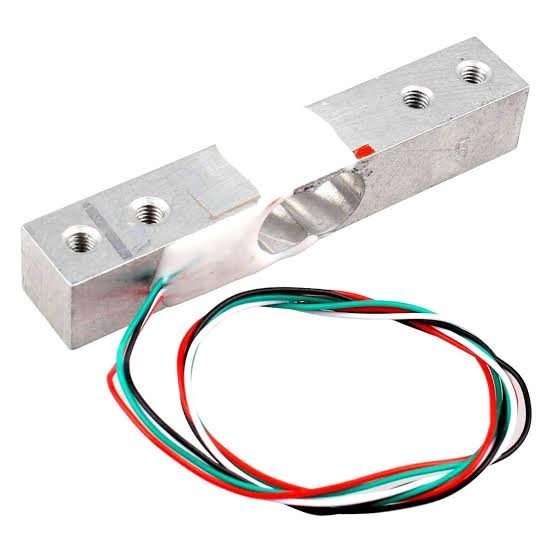
\includegraphics[
        height=5cm,  % Fixed height for both images
        angle=0,
        trim={0.5cm 0.3cm 0.5cm 0.3cm},
        clip
    ]{projects_records/Load_cell/Images/load_cell.png}
\end{minipage}
\hfill
\begin{minipage}{0.45\textwidth}
    \centering
    \includegraphics[
        height=5cm,  % Same height as first image
        angle=0,
        trim={0.5cm 0.3cm 0.5cm 0.3cm},
        clip
    ]{projects_records/Load_cell/Images/load_cell2.png}  % Change to second image
\end{minipage}
\caption{1\,kg Single-Point Load Cell (Front and Back View)}
\label{fig:loadcell}
\end{figure}

%%%%%%%%%%%%%%%%%%%%%%%%%%%%%%%%%%%%%%%%%%%%%%%%%%%%%%%%%%%%%%%%%%%%%%%

\subsection{HX711 Load Cell Amplifier Module}

The electrical signal generated by the load cell is extremely small and cannot be measured directly by the ESP32. Therefore, an HX711 precision amplifier module was used between the load cell and the microcontroller.

The HX711 amplifies the low-level signal produced by the load cell and converts it into a high-resolution digital value that can be processed by the ESP32. It is specifically designed for weighing applications and provides excellent measurement stability and resolution. \cite{hx711_datasheet}

The module communicates with the ESP32 using only two digital pins, making hardware interfacing simple while maintaining high measurement accuracy.

Figure~\ref{fig:hx711} shows the HX711 module used in this project.

\begin{figure}[H]
\centering
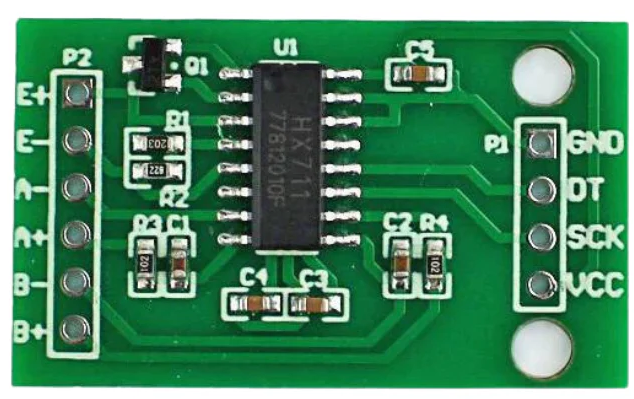
\includegraphics[width=0.25\textwidth]{projects_records/Load_cell/Images/hx711_module.png}
\caption{HX711 Load Cell Amplifier Module}
\label{fig:hx711}
\end{figure}

%%%%%%%%%%%%%%%%%%%%%%%%%%%%%%%%%%%%%%%%%%%%%%%%%%%%%%%%%%%%%%%%%%%%%%%

\subsection{ESP32 Dev Module} 

The ESP32 Dev Module acts as the central processing unit of the weighing system. It receives the digital data from the HX711 module, performs calibration and tare correction, calculates the actual weight, and updates the OLED display continuously. 

The ESP32 was selected instead of a conventional microcontroller because it offers higher processing capability, larger memory, built-in Wi-Fi and Bluetooth connectivity, and sufficient GPIO pins for future expansion. \cite{esp32_datasheet}

Although wireless communication was not implemented in the final system, the availability of integrated Wi-Fi provides flexibility for future Internet of Things (IoT) applications such as remote monitoring and cloud-based data logging.

Figure~\ref{fig:esp32} shows the ESP32 development board used during this project.

\begin{figure}[H]
\centering
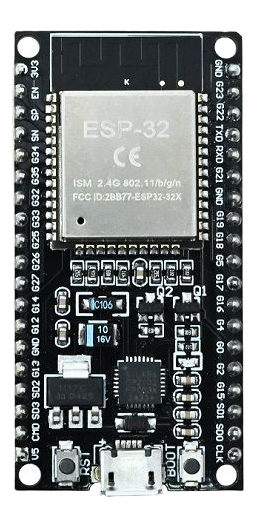
\includegraphics[
    width=0.20\textwidth,
    angle=90,
    trim={1cm 2cm 1cm 2cm},
    clip
]{projects_records/Load_cell/Images/1165429-2-removed-bg.png}

\caption{ESP32 Dev Module}
\label{fig:esp32}
\end{figure}
%%%%%%%%%%%%%%%%%%%%%%%%%%%%%%%%%%%%%%%%%%%%%%%%%%%%%%%%%%%%%%%%%%%%%%%

\subsection{SH1106 OLED Display}

A 1.3-inch SH1106 OLED display was used to provide a real-time visual indication of the measured weight.

After every measurement cycle, the ESP32 updates the display with the latest weight value. During the calibration and sensitivity experiments, all observations were recorded only after the displayed value became stable.

The OLED display offers good contrast, low power consumption, and excellent readability, making it suitable for standalone operation without requiring continuous observation of the Serial Monitor. \cite{sh1106_datasheet}

Figure~\ref{fig:oled} shows the OLED display used in the developed weighing system.

\begin{figure}[H]
\centering
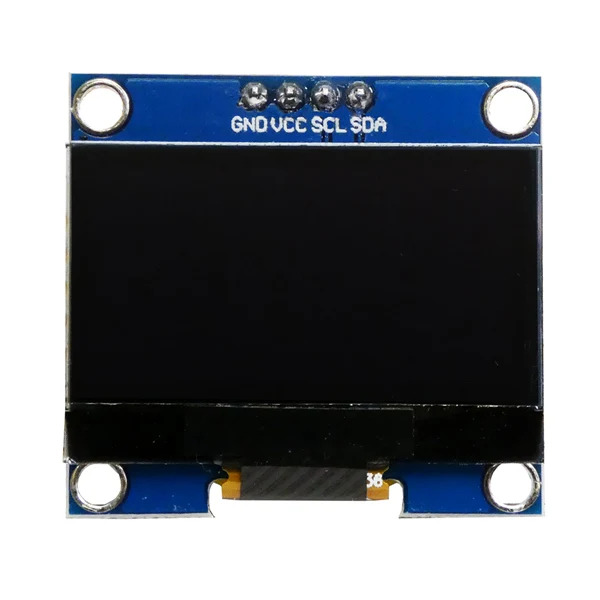
\includegraphics[width=0.25\textwidth]{projects_records/Load_cell/Images/oled.jpg}
\caption{SH1106 OLED Display}
\label{fig:oled}
\end{figure}

%%%%%%%%%%%%%%%%%%%%%%%%%%%%%%%%%%%%%%%%%%%%%%%%%%%%%%%%%%%%%%%%%%%%%%%
%%%%%%%%%%%%%%%%%%%%%%%%%%%%%%%%%%%%%%%%%%%%%%%%%%%%%%%%%%%%%%%%%%%%%%%

\section{Hardware Connections and Circuit Implementation}

After selecting the required hardware components, the hardware prototype was assembled by interfacing the load cell with the HX711 amplifier module, the ESP32 Dev Module, and the SH1106 OLED display. Careful wiring of each component was necessary to ensure reliable communication and accurate weight measurement.

The complete hardware implementation consists of three major interfaces:

\begin{enumerate}
    \item Load Cell to HX711 Module
    \item HX711 Module to ESP32 Dev Module
    \item SH1106 OLED Display to ESP32 Dev Module
\end{enumerate}

%%%%%%%%%%%%%%%%%%%%%%%%%%%%%%%%%%%%%%%%%%%%%%%%%%%%%%%%%%%%%%%%%%%%%%%

\subsection{Hardware Components}

Table~\ref{tab:hardware_components} lists the hardware used to develop the weighing system.

\begin{table}[H]
\centering
\caption{Hardware Components Used}
\label{tab:hardware_components}

\begin{tabular}{|p{8cm}|c|}
\hline
\textbf{Component} & \textbf{Quantity} \\
\hline
ESP32 Dev Module & 1 \\
1\,kg Single-Point Load Cell & 1 \\
HX711 Load Cell Amplifier Module & 1 \\
1.3-inch SH1106 OLED Display & 1 \\
USB Cable & 1 \\
Connecting Wires & As Required \\
Breadboard (Testing Stage) & 1 \\
Laptop / Computer & 1 \\
Commercial Digital Weighing Scale & 1 \\
\hline
\end{tabular}

\end{table}

%%%%%%%%%%%%%%%%%%%%%%%%%%%%%%%%%%%%%%%%%%%%%%%%%%%%%%%%%%%%%%%%%%%%%%%

\subsection{Load Cell to HX711 Connections}

The load cell is connected directly to the HX711 amplifier through four wires. These wires provide power to the Wheatstone bridge inside the load cell and transfer the differential output signal to the amplifier.

\begin{table}[H]
\centering
\caption{Load Cell Connections}
\label{tab:loadcell_connection}

\begin{tabular}{|c|c|p{7cm}|}
\hline
\textbf{Wire Colour} & \textbf{HX711 Pin} & \textbf{Purpose} \\
\hline
Red & E+ & Positive excitation voltage \\
Black & E-- & Ground / Negative excitation \\
Green & A+ & Positive signal output \\
White & A-- & Negative signal output \\
\hline
\end{tabular}

\end{table}

%%%%%%%%%%%%%%%%%%%%%%%%%%%%%%%%%%%%%%%%%%%%%%%%%%%%%%%%%%%%%%%%%%%%%%%

\subsection{HX711 to ESP32 Connections}

The HX711 communicates digitally with the ESP32 using only two GPIO pins. Power is supplied directly from the ESP32 development board.

\begin{table}[H]
\centering
\caption{HX711 to ESP32 Connections}
\label{tab:hx711_esp32}

\begin{tabular}{|c|c|}
\hline
\textbf{HX711 Pin} & \textbf{ESP32 Pin} \\
\hline
VCC & 3.3V \\
GND & GND \\
DT (DOUT) & GPIO 32 \\
SCK & GPIO 26 \\
\hline
\end{tabular}

\end{table}

%%%%%%%%%%%%%%%%%%%%%%%%%%%%%%%%%%%%%%%%%%%%%%%%%%%%%%%%%%%%%%%%%%%%%%%

\subsection{SH1106 OLED to ESP32 Connections}

The SH1106 OLED display communicates with the ESP32 through the I\textsuperscript{2}C interface.

\begin{table}[H]
\centering
\caption{SH1106 OLED Connections}
\label{tab:oled_connection}

\begin{tabular}{|c|c|}
\hline
\textbf{OLED Pin} & \textbf{ESP32 Pin} \\
\hline
VCC & 3.3V \\
GND & GND \\
SDA & GPIO 21 \\
SCL & GPIO 22 \\
\hline
\end{tabular}

\end{table}

%%%%%%%%%%%%%%%%%%%%%%%%%%%%%%%%%%%%%%%%%%%%%%%%%%%%%%%%%%%%%%%%%%%%%%%

\subsection{Complete Circuit Diagram}

Figure~\ref{fig:circuit} illustrates the complete circuit diagram of the developed weighing system.

\begin{figure}[H]
\centering
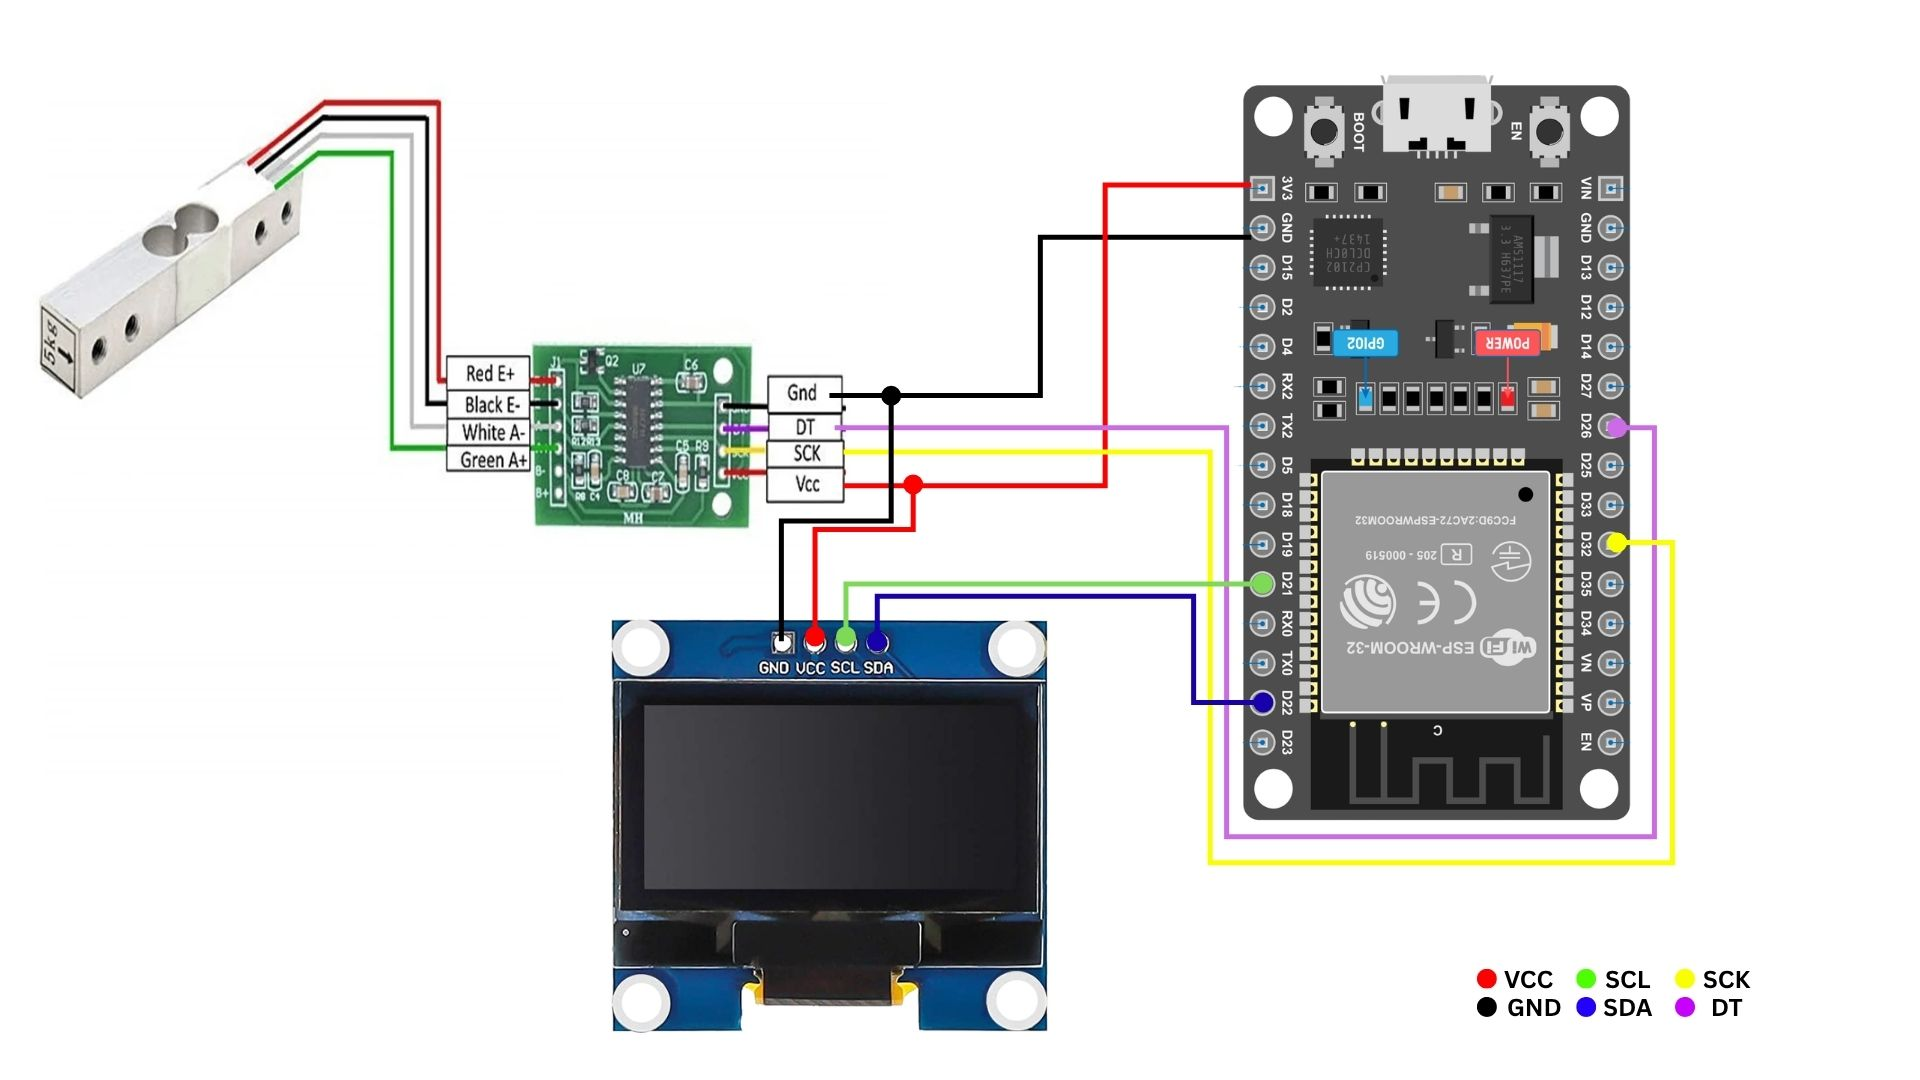
\includegraphics[width=0.90\textwidth]{projects_records/Load_cell/Images/circuit_hardware.jpg}
\caption{Complete Circuit Diagram of the Developed Weighing System}
\label{fig:circuit}
\end{figure}

%%%%%%%%%%%%%%%%%%%%%%%%%%%%%%%%%%%%%%%%%%%%%%%%%%%%%%%%%%%%%%%%%%%%%%%

\subsection{Experimental Hardware Setup}

After completing the wiring, the entire system was assembled on the laboratory workbench. The load cell was securely mounted to minimize mechanical vibration during measurements, while the HX711 module and ESP32 were connected using jumper wires. The SH1106 OLED display was positioned for easy observation of the measured weight during calibration and sensitivity testing.

Figure~\ref{fig:hardware_setup} shows the actual hardware setup developed during the internship.

\begin{figure}[H]
\centering

\begin{minipage}{0.48\textwidth}
\centering
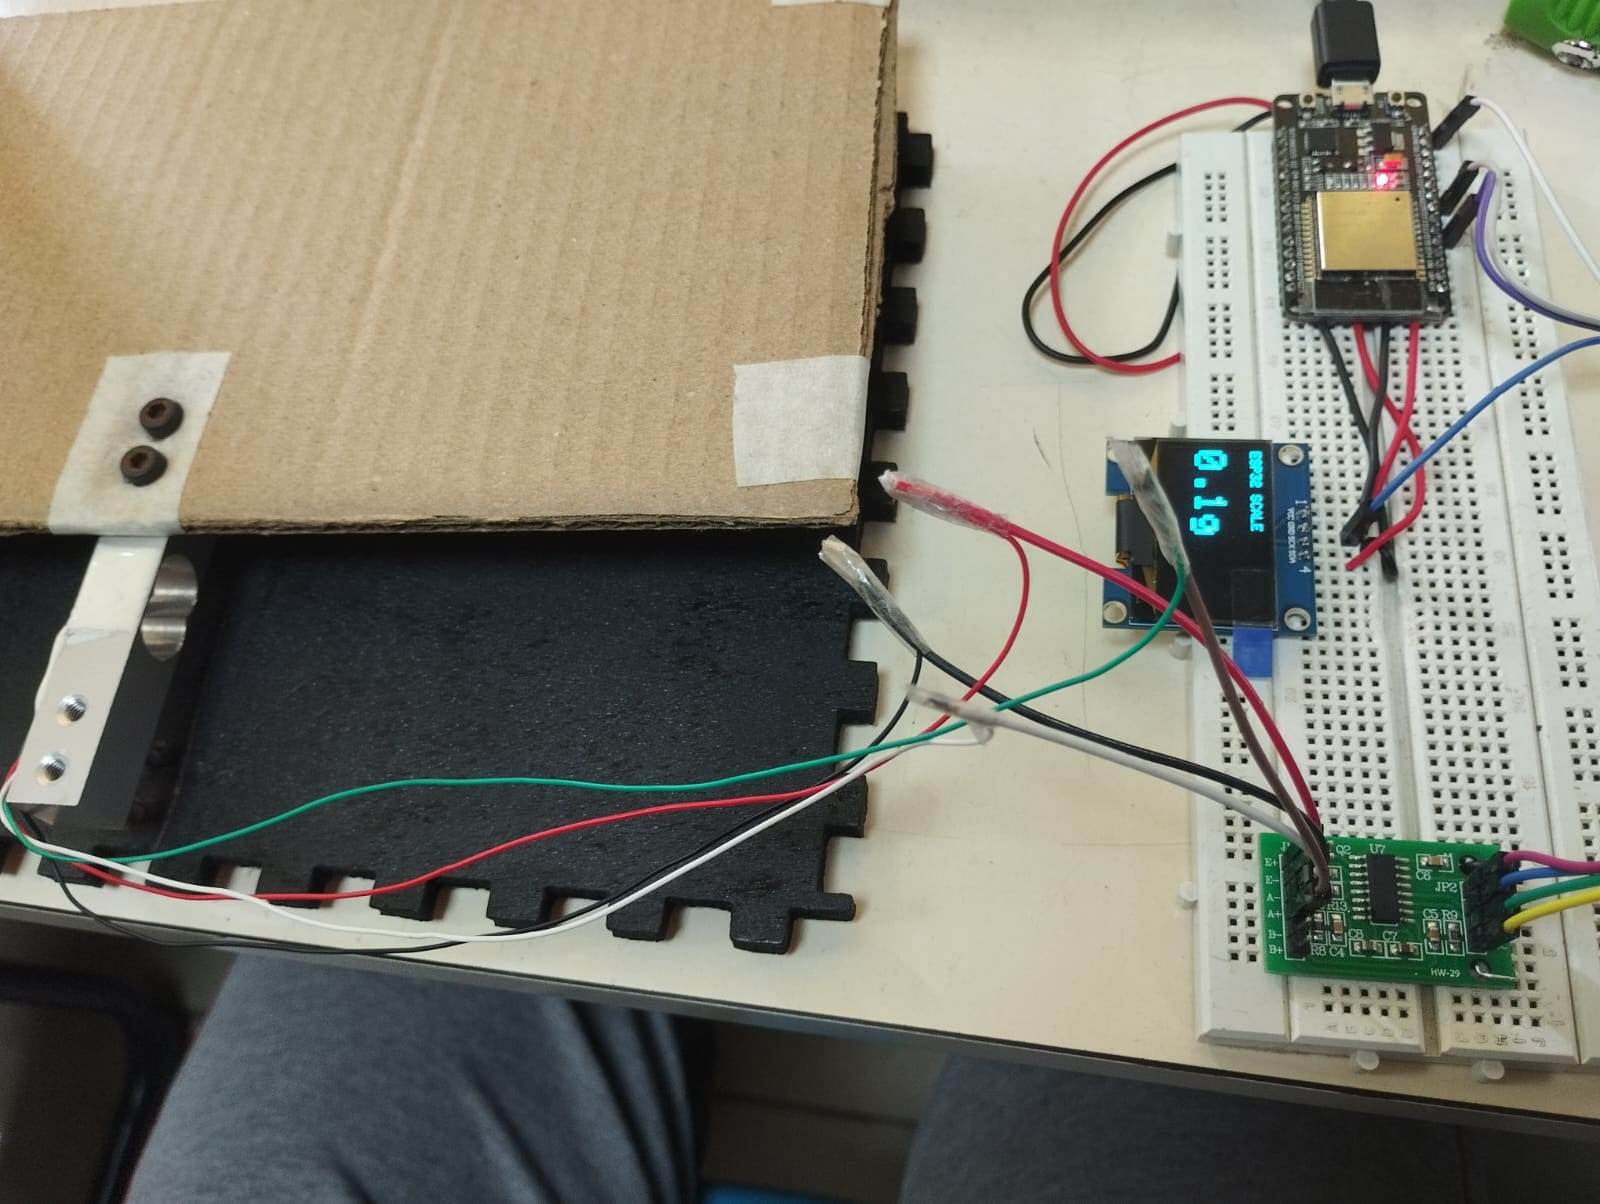
\includegraphics[width=\linewidth]{projects_records/Load_cell/Images/Complete_setup.jpeg}
\caption{Complete Experimental Setup}
\end{minipage}
\hfill
\begin{minipage}{0.48\textwidth}
\centering
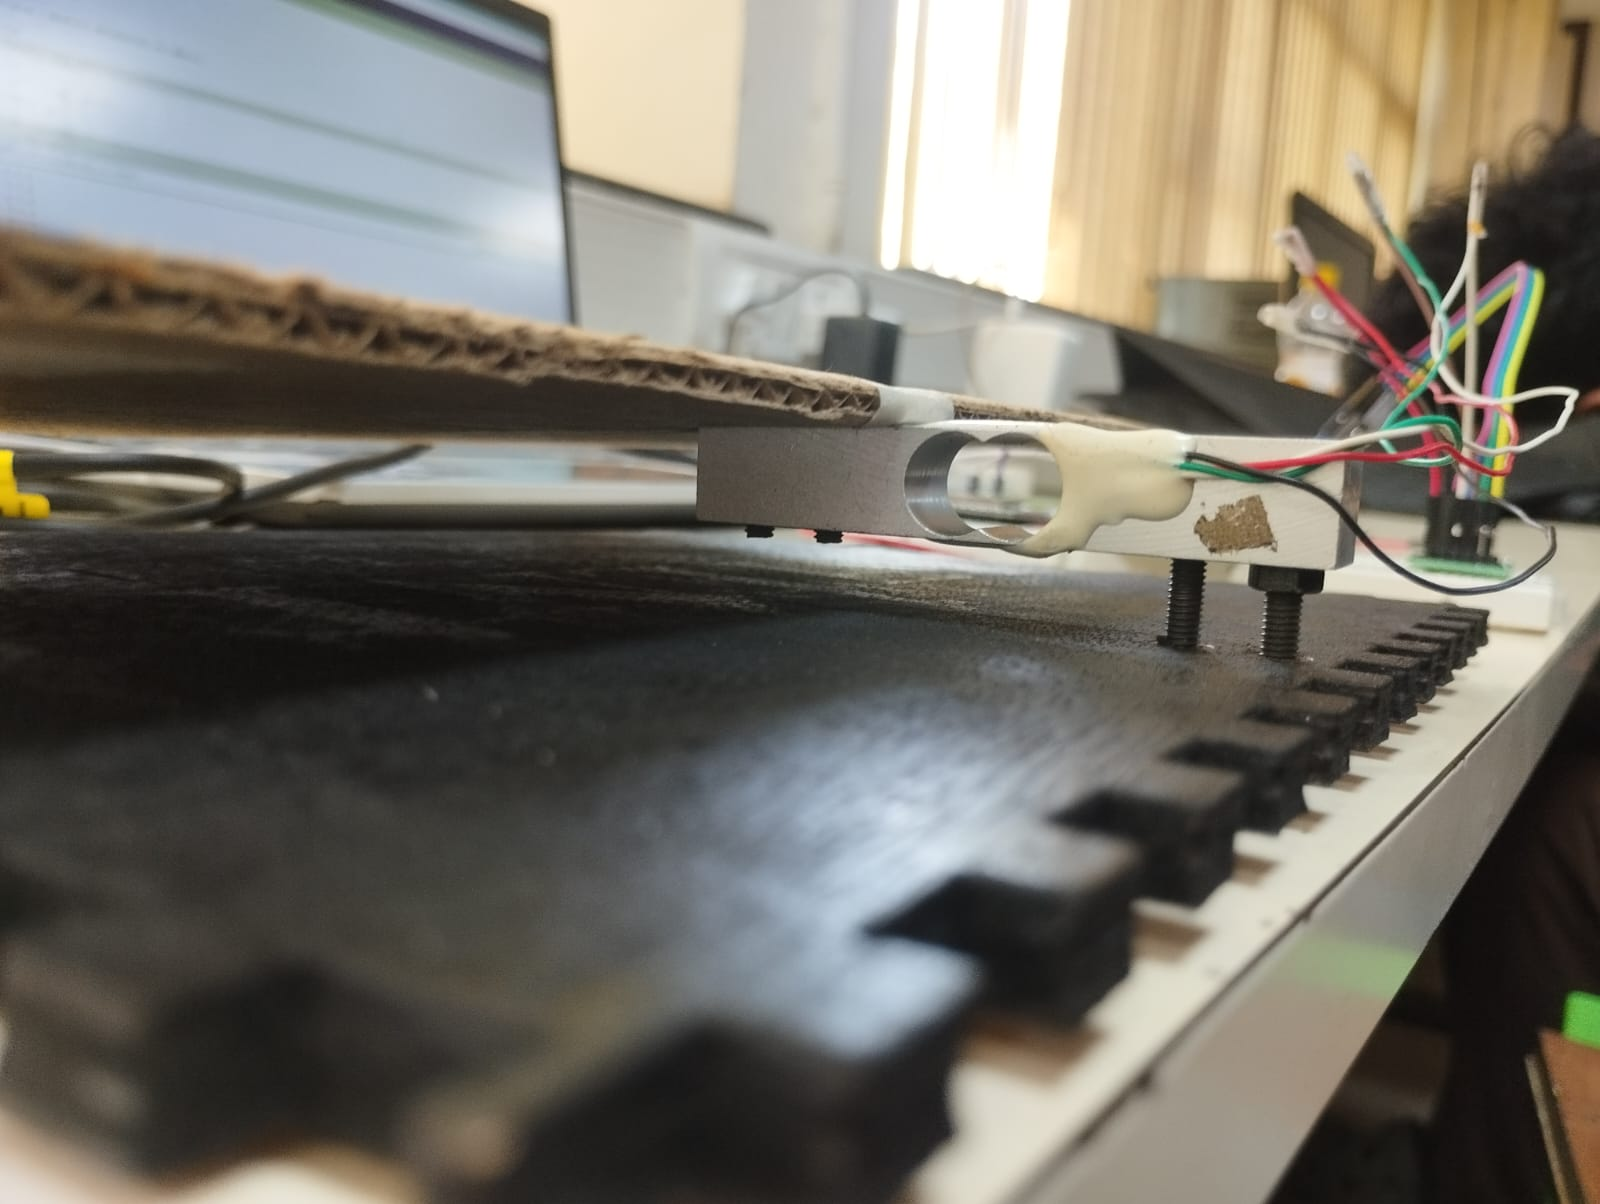
\includegraphics[width=\linewidth]{projects_records/Load_cell/Images/Structure.jpeg}
\caption{Mounted Load Cell and Platform}
\end{minipage}

\caption{Hardware Setup Used During Experimental Evaluation}
\label{fig:hardware_setup}

\end{figure}

%%%%%%%%%%%%%%%%%%%%%%%%%%%%%%%%%%%%%%%%%%%%%%%%%%%%%%%%%%%%%%%%%%%%%%%

\section{Software Implementation}

Firmware for the smart weighing system was written using the Arduino IDE with the ESP32 Dev Module as the target development board. The program is responsible for acquiring data from the HX711 module, processing the measured values, applying calibration, and displaying the final weight on the SH1106 OLED display.

During operation, the ESP32 continuously reads the digital output of the HX711 module, calculates the corresponding weight, and refreshes the OLED display in real time. To improve measurement stability, multiple sensor readings are averaged before displaying the final value.

%%%%%%%%%%%%%%%%%%%%%%%%%%%%%%%%%%%%%%%%%%%%%%%%%%%%%%%%%%%%%%%%%%%%%%%

\subsection{Software Tools Used}


The software and libraries used during the project's development are listed in Table~\ref{tab:software}. \cite{arduino_ide,hx711_library,adafruit_gfx,adafruit_sh110x}


\begin{table}[H]

\centering
\caption{Software Development Tools}
\label{tab:software}

\begin{tabular}{|p{6cm}|p{7cm}|}
\hline
\textbf{Software / Library} & \textbf{Purpose} \\
\hline
Arduino IDE & Program development and uploading firmware \\
ESP32 Board Package & ESP32 board support \\
HX711 Library & Reading weight from the load cell \\
Adafruit SH110X Library & OLED display interface \\
Adafruit GFX Library & Graphics and text display \\
Serial Monitor & Calibration and debugging \\
\hline
\end{tabular}

\end{table}

%%%%%%%%%%%%%%%%%%%%%%%%%%%%%%%%%%%%%%%%%%%%%%%%%%%%%%%%%%%%%%%%%%%%%%%

\subsection{Calibration of the Load Cell}

The load cell does not directly provide weight in grams. Instead, the HX711 module produces a raw digital output that is proportional to the applied load. Therefore, calibration is required to establish the relationship between the raw sensor output and the actual weight.

The calibration process was performed experimentally using a commercial digital weighing scale as the reference instrument. Initially, the raw output of the load cell was recorded without placing any object on the weighing platform. To reduce the effect of measurement noise, the average of multiple raw readings was considered as the zero-load reference value.

A known weight was then measured using the digital weighing scale and placed on the load cell platform. After allowing the readings to stabilize, the average of multiple raw readings was recorded again.
The calibration factor was estimated using the relationship
\begin{equation}
\text{Calibration Factor}=
\frac{\text{Signal with Test Weight}-\text{Signal at Zero}}
{\text{Known Test Weight}}
\label{eq:calibration}
\end{equation}

where

\begin{itemize}
\item Signal at Zero is the average raw value measured with no applied load.
\item Signal with Test Weight is the average raw value measured after placing the known weight.
\item Known Test Weight is the reference weight measured using the commercial digital weighing scale.
\end{itemize}

\thispagestyle{githubpage}

\thispagestyle{githubpage}

\subsection{Program Workflow}

The calculated value provided an initial estimate of the calibration factor.
The weight displayed on the Serial Monitor was compared with the reference weight. If the measured value differed from the reference, the calibration factor was adjusted, and the experiment was repeated until both values agreed closely.

Once the appropriate calibration factor was obtained, it was incorporated into the weighing system's final firmware.

The firmware follows a simple sequence of operations during execution.

\begin{algorithm}[H]
\caption{Firmware Execution}
\begin{algorithmic}[1]

\Function{setup}{}
    \State Initialize ESP32
    \State Initialize HX711 module
    \State Initialize SH1106 OLED display
    \State Load calibration factor
    \State Perform tare operation
\EndFunction

\Function{loop}{}
    \State Read weight data from the HX711 module
    \State Average multiple sensor readings
    \State Calculate the weight
    \State Display the measured weight on the OLED display
    \State Send the measured weight to the Serial Monitor
\EndFunction

\end{algorithmic}
\end{algorithm}

%Figure~\ref{fig:software_flow} shows the overall Program workflow.

% \begin{figure}[H]
% \centering
% 
\includegraphics[width=1\textwidth]{projects_records/Load_cell/Images/Program Workflow (1).png}
% \caption{Program Workflow}
% \label{fig:software_flow}
% \end{figure}

%%%%%%%%%%%%%%%%%%%%%%%%%%%%%%%%%%%%%%%%%%%%%%%%%%%%%%%%%%%%%%%%%%%%%%%

\subsection{Weight Measurement}

The HX711 library is used to obtain the weight measurements from the load cell. Instead of using a single sensor reading, the ESP32 averages twenty consecutive readings before calculating the displayed weight. This averaging technique reduces random fluctuations and provides a more stable measurement.

After processing the measured data, the calculated weight is displayed in grams on the SH1106 OLED.

%%%%%%%%%%%%%%%%%%%%%%%%%%%%%%%%%%%%%%%%%%%%%%%%%%%%%%%%%%%%%%%%%%%%%%%

\subsection{Program Source Code}

The complete source code is available in the GitHub repository, and the repository link is provided in the footer of this report.
\thispagestyle{githubpage}
%%%%%%%%%%%%%%%%%%%%%%%%%%%%%%%%%%%%%%%%%%%%%%%%%%%%%%%%%%%%%%%%%%%%%%%

\section{Testing Methodology and Experimental Results}

After completing the hardware assembly, software implementation, and calibration of the weighing system, experiments were conducted to evaluate its sensitivity and measurement accuracy.

A container containing approximately \textbf{100 g} of water was first weighed using a commercial digital weighing scale and then placed on the load cell platform. This initial weight served as the reference value throughout the experiment.

To investigate the minimum detectable change in weight, approximately \textbf{1 mL} of water was removed from the container using a syringe at regular intervals of about \textbf{15--20 minutes}. Since the density of water is approximately \textbf{1 g/mL}, each removal produced a weight reduction of nearly \textbf{1 g}.

After each removal, the weighing system was allowed to stabilize before recording the displayed weight from the SH1106 OLED display. Waiting for a stable reading minimized the influence of temporary fluctuations caused by mechanical vibrations and sensor settling.

The measured weight displayed by the developed system was then compared with the expected weight after each 1 mL reduction. This procedure was repeated several times to evaluate the sensitivity, accuracy, and repeatability of the developed weighing system.

The complete experimental procedure is summarized below:

\begin{enumerate}
    \item Measure approximately 100 g of water using a commercial digital weighing scale.
    \item Place the container on the calibrated load cell platform.
    \item Wait until the displayed weight becomes stable and record the initial reading.
    \item Remove approximately 1 mL of water using a syringe.
    \item Wait again until the displayed weight stabilizes.
    \item Record the new weight displayed on the OLED.
    \item Compare the measured value with the expected weight.
    \item Repeat the procedure several times to evaluate the sensitivity and accuracy of the system.
\end{enumerate}

%%%%%%%%%%%%%%%%%%%%%%%%%%%%%%%%%%%%%%%%%%%%%%%%%%%%%%%%%%%%%%%%%%%%%%%
\section{Observation Table}
After completing the calibration process, The prototype weighing system was evaluated to determine its sensitivity and measurement accuracy. A container containing approximately 100\,g of water was placed on the load cell platform. Subsequently, approximately 1\,mL of water was removed using a syringe at regular intervals of 15 \& 20 minutes.

Since the density of water is approximately 1\,g/mL, each removal resulted in an expected decrease of nearly 1\,g in the total weight. After every removal, the displayed weight on the SH1106 OLED was allowed to stabilize before recording the observation. After every removal, the system was allowed to stabilize before recording the displayed weight from the SH1106 OLED display.

The observed readings are presented in Table~\ref{tab:observation} \& Table~\ref{tab:sensitivity_test}.

\begin{table}[H]
\centering
\caption{Data Recorded Every 15 Minutes}
\label{tab:observation}

\begin{tabular}{|c|c|c|c|c|}
\hline
\textbf{S.No.} &
\textbf{Elapsed} &
\textbf{Water Removed} &
\textbf{Measured Weight} &
\textbf{Rounded} \\

&
\textbf{(min)} &
\textbf{(mL)} &
\textbf{(g)} &
\textbf{Weight (g)}\\
\hline

1 & 0  & 0 & 100.02 & 100 \\
2 & 15 & 1 & 98.94  & 99 \\
3 & 30 & 1 & 97.33  & 97 \\
4 & 45 & 1 & 94.91  & 95 \\
5 & 60 & 1 & 92.72  & 93 \\
6 & 75 & 1 & 90.97  & 91 \\
7 & 90 & 1 & 89.31  & 89 \\
\hline

\end{tabular}
\end{table}

%%%%%%%%%%%%%%%%%%%%%%%%%%%%%%%%%%%%%%%%%%%%%%%%%%%%%%%%%%%%%%%%%%%%%%%

\begin{table}[H]
\centering
\caption{Data Recorded Every 20 Minutes}
\label{tab:sensitivity_test}

\renewcommand{\arraystretch}{1.15}
\setlength{\arrayrulewidth}{0.6pt}

\begin{tabular}{|c|c|c|c|c|}
\hline
\textbf{S.No.} &
\textbf{Elapsed Time} &
\textbf{Water Removed} &
\textbf{Measured Weight} &
\textbf{Rounded Weight} \\

&
\textbf{(min)} &
\textbf{(mL)} &
\textbf{(g)} &
\textbf{(g)} \\
\hline

1  & 0   & 0 & 100.28 & 100 \\
2  & 20  & 1 & 98.96  & 99  \\
3  & 40  & 1 & 97.58  & 98  \\
4  & 60  & 1 & 95.72  & 96  \\
5  & 80  & 1 & 93.84  & 94  \\
6  & 100 & 1 & 92.72  & 93  \\
7  & 120 & 1 & 90.74  & 91  \\
8  & 140 & 1 & 89.09  & 89  \\
9  & 160 & 1 & 87.78  & 88  \\
10 & 180 & 1 & 85.88  & 86  \\
11 & 200 & 1 & 83.95  & 84  \\
12 & 220 & 1 & 82.15  & 82  \\
13 & 240 & 1 & 81.27  & 81  \\
14 & 260 & 1 & 79.46  & 79  \\
15 & 280 & 1 & 77.75  & 78  \\
16 & 300 & 1 & 76.25  & 76  \\
17 & 320 & 1 & 75.49  & 75  \\
18 & 340 & 1 & 73.92  & 74  \\
\hline

\end{tabular}
\end{table}
%%%%%%%%%%%%%%%%%%%%%%%%%%%%%%%%%%%%%%%%%%%%%%%%%%%%%%%%%%%%%%%%%%%%%%%

The data presented in Table~\ref{tab:observation}  \& Table~\ref{tab:sensitivity_test} demonstrate that the developed weighing system was capable of detecting small reductions in weight produced by the removal of approximately 1\,mL of water during each observation. The measured values closely followed the expected trend throughout the experiment.

Minor deviations between the expected and measured weights were observed due to sensor noise, mechanical vibrations, and environmental factors. However, the absolute error remained within an acceptable range for the entire measurement period. Recording measurements only after the OLED display value became stable and averaging multiple sensor readings significantly improved the system's repeatability and stability.

These observations confirm that the developed weighing system is sufficiently sensitive to detect weight variations of approximately 1\,g, demonstrating the effectiveness of the calibration procedure and the overall performance of the load cell, HX711 module, and ESP32-based measurement system.

%%%%%%%%%%%%%%%%%%%%%%%%%%%%%%%%%%%%%%%%%%%%%%%%%%%%%%%%%%%%%%%%%%%%%%%
%%%%%%%%%%%%%%%%%%%%%%%%%%%%%%%%%%%%%%%%%%%%%%%%%%%%%%%%%%%%%%%%%%%%%%%

\section{Results and Discussion}

The sensitivity evaluation demonstrated that the weighing system reliably detected small variations in weight throughout the experiment. A consistent decrease in measured weight was observed after each withdrawal of approximately \textbf{1~mL} of water, confirming that the system responded appropriately to incremental changes in load. This behavior indicates that the integration of the \textbf{load cell}, \textbf{the HX711 amplifier} and \textbf{the ESP32 microcontroller} provided an effective and reliable weight measurement.

The recorded measurements exhibited a clear decreasing trend that closely matched the expected reduction in water mass. Although minor fluctuations were present between successive readings, these variations remained small and did not affect the overall consistency of the results. Such fluctuations are expected in practical sensing systems due to \emph{electrical noise}, \emph{environmental disturbances}, and the high sensitivity of strain-gauge-based load cells.

Measurement stability was significantly improved by averaging \textbf{20 consecutive sensor readings} before displaying the final value. This averaging technique effectively minimized random noise and reduced the influence of small mechanical vibrations, resulting in smoother and more repeatable measurements. In addition, data were recorded only after the OLED display reached a stable value, ensuring consistency across all observations.

The experiment also highlighted certain practical limitations associated with manual operation. Accurately withdrawing exactly \textbf{1~mL} of water using a syringe during each trial was challenging, leading to small variations in the actual quantity removed. Consequently, slight differences between the expected and measured weights were observed. These deviations are primarily attributed to \textbf{human handling errors} rather than limitations of the sensing hardware or measurement algorithm.

Overall, the sensitivity test confirmed that the developed weighing system could successfully detect weight changes of approximately \textbf{1~g}, corresponding to nearly \textbf{1~mL} of water. The experimental results demonstrate that the system provides \textbf{stable}, \textbf{repeatable}, and \textbf{sufficiently accurate} measurements within the operating range of the \textbf{1~kg load cell}. These findings validate the effectiveness of the proposed design for applications requiring \textbf{real-time monitoring of small weight variations} and demonstrate its potential for deployment in \emph{laboratory experiments}, \emph{industrial monitoring}, and \emph{IoT-based sensing applications}.


%%%%%%%%%%%%%%%%%%%%%%%%%%%%%%%%%%%%%%%%%%%%%%%%%%%%%%%%%%%%%%%%%%%%%%%

%%%%%%%%%%%%%%%%%%%%%%%%%%%%%%%%%%%%%%%%%%%%%%%%%%%%%%%%%%%%%%%%%%%%%%%

\section{Future Scope}

Although the proposed weighing system successfully measures weight with good sensitivity and stability, several improvements can further enhance its functionality and practical applications.

\begin{itemize}

\item \textbf{Automatic Data Logging:} The current system displays the measured weight on the SH1106 OLED display. In future, the ESP32 can automatically transmit every measured reading to a cloud database without requiring manual recording.

\item \textbf{Backend Database Integration:} The weighing system can be integrated with a backend server using technologies such as Node.js and PostgreSQL. This would enable secure storage of historical weight measurements along with timestamps for future analysis.

\item \textbf{Real-Time Web Dashboard:} The stored data can be processed and visualized through a web-based dashboard. Platforms such as Grafana can be integrated with the database to display live weight measurements, historical trends, statistical summaries, and interactive graphs.

\item \textbf{Remote Monitoring:} Since the ESP32 provides built-in Wi-Fi connectivity, the developed system can be extended for remote monitoring, allowing users to observe weight measurements from any location through a web application.

\item \textbf{Alert and Notification System:} Automatic notifications can be generated whenever the measured weight exceeds or falls below predefined threshold values. Such alerts can be delivered through email, SMS, or mobile applications.

\item \textbf{Industrial and IoT Applications:} The developed system can be integrated into industrial automation, smart inventory management, laboratory monitoring, and Internet of Things (IoT) applications where continuous weight monitoring and automatic data collection are required.

\end{itemize}

%%%%%%%%%%%%%%%%%%%%%%%%%%%%%%%%%%%%%%%%%%%%%%%%%%%%%%%%%%%%%%%%%%%%%%%
